
\label{cha:circle}

An effective principle in mathematics is that when you want to study a certain 
phenomenon you should search for a single type that captures this phenomenon.  
Here are two examples
\begin{enumerate}
\item The contractible type $\bn 1$ has the property that given 
\emph{any} type $A$ a function $\bn 1\to A$ provides exactly the 
same information as picking an element in $A$: 
the function $A\to (\bn 1\to A)$ sending $a:A$ to the 
constant function with value $a$ is an equivalence, \ie $A=(\bn 1\to A)$.
\item The type $\Prop$ of propositions has the property that 
given \emph{any} type $A$ a function $A\to\Prop$ provides exactly 
the same information as picking a subtype of $A$.
\end{enumerate}
We are interested in symmetries, and so we should search for a type $X$ which is so that given \emph{any} type $A$ the type of functions $X\to A$ (or $A\to X$, but that's not what we're going to do) picks out exactly the symmetries in $A$.  We will soon see that there is such a type: the circle which is built \emph{exactly} so that this ``universality with respect to symmetries'' holds.  It may be surprising to see how little it takes to define it; especially in hindsight when we eventually discover some the many uses of the circle.

A symmetry in $A$ is an identity $p:a=_Aa$ for some $a:A$.  
Now, we can take any iteration of $p$ (composing $p$ with itself a number of times), 
and we can consider the inverse $p^{-1}$ and \emph{its} iterations.  
So, by giving one symmetry we at the same time give a lot of symmetries.  
For a particular $p$ it may be that not all of the iterations are different, 
for instance it may be that $p^2=p^0\defequi\refl a$ (like in \cref{xca:C2}), 
or even more dramatic: if  $p=\refl a$, then \emph{all} the iterates of $p$ are equal. 
However, in general we must be prepared that all the powers of $p$ 
(positive, $0$ and negative) are distinct. 
Hence, the circle must have a distinct symmetry for every integer. 
We would have enjoyed defining the integers this way, 
but being that ideological would be somewhat inefficient. 
Hence we give a more hands-on approach defining the circle 
and the integers separately. Thereafter we prove that the type of 
symmetries of the circle is equivalent to the set of integers. 

\section{The circle and its universal property}
\label{sec:S1}

Recall the definition of propositional truncation from \cref{sec:prop-trunc}.
The circle is another example of a \emph{higher inductive type},
see \cite[Ch. 6]{hottbook} for more information.

\begin{definition}
  \label{def:circle}
The circle is a type $\Sc:\UU$ with an element (constructor) $\base : \Sc$ and 
an identification (constructor) $\Sloop: \base=\base$. For convenience and
clarity the (higher) induction principle for $\Sc$ is explained
by first stating a recursion principle for $\Sc$.

Let $A$ be a type. In order to define a function $f:\Sc\to A$,
it suffices to give an element $a$ of $A$ together with an
identification $l$ of type $a=a$. The function $f$ defined
by this data satisfies $f(\base)\jdeq a$ and $\ap{f}(\Sloop)=l$.

Let $A(x)$ be a type for every $x:\Sc$. The induction principle of $\Sc$
states that, in order to prove $A(x)$ for every element $x$ of $\Sc$,
it suffices to give an element $a$ of $A(\base)$ together with an
identification $l$ of type $\trp{A,\Sloop}(a) = a$. More precisely,
giving such $a$ and $l$ defines a function $f:\prod_{x:\Sc}T(x)$ such that
$f(\base)\jdeq a$ and $\apd{f}(\Sloop)=l$. 
\end{definition}

Giving $a$ as above is referred to as `the base case', and
giving $l$ as `the loop case'.
As promised, we now demonstrate that a function from the circle exactly 
picks out an element and a symmetry of that element:

\begin{lemma}\label{lem:freeloopspace}
For all types $A$, the evaluation function 
\[
\ev_A : (\Sc\to A)\to \sum_{a:A}(a=_Aa)\text{~defined by~} 
\ev_A(g)\defeq (g(\base),g(\Sloop))
\]
is an equivalence, with inverse $\el_A$ defined by the recursion principle.  
%In particular, if $a:A$, the function $((\Sc,\base)\to_* (A,a))\to (a=_Aa)$ 
%given by sending $g:\Sc\to A$ to $g(\Sloop)$ is an equivalence. 
\end{lemma}
\begin{proof}
Fix $A:\UU$. We apply \cref{lem:weq-iso}. 
For all $a:A$ and $l:a=a$ we have $\ev(\el(a,l))=(a,l)$
by the recursion principle. It remains to prove
$\el(\ev(f))=f$ for all $f:\Sc\to A$. This will follow
from the following more general result. Assume 
$p: f(\base)= g(\base)$ and $q: f(\Sloop) = p^{-1}\cdot g(\Sloop)\cdot p$.
We show $f=g$, for which it suffices to prove by circle induction
that $P(x)\defeq(f(x)=g(x))$ for all $x:\Sc$.
For the base case we take $p$.
For the loop case we have to show $\trp{P,\Sloop}(p)=p$.
By \cref{lem:trp-in-fx=Ygx} we have 
$\trp{P,\Sloop}(p)=g(\Sloop)\cdot p \cdot f(\Sloop)^{-1}$. 
By $q$ we have $g(\Sloop) = p\cdot f(\Sloop) \cdot p^{-1}$.
Hence $\trp{P,\Sloop}(p)=p$ by easy calculation.
To finally get $\el(\ev(f))=f$,
note that $\ev(\el(\ev(f)))=(f(\base),f(\Sloop))$ with $p\defeq\refl{f(\base)}$
and $q$ coming from the induction principle.
\end{proof}

\begin{remark}
A function $f:\Sc\to A$ is often called a \emph{loop} in $A$, 
the picture being that $f$ throws $\Sloop:\base=\base$ as a lasso in the type $A$.

  Under univalence, so that $a=_Aa$ is identified with the pointed functions 
from the circle, this allows for a very graphic interpretation of the 
symmetries in $a=_Aa$: they are all in the image of a function $g$ from 
the circle: they are loops in the type $A$ starting and ending at $a$! ((picture!!))
\end{remark}

\begin{lemma}\label{lem:circleisconnected}
  The circle is connected.
\end{lemma}
\begin{proof}
We show $\Trunc{\base=z}$ for all $z:\Sc$ by circle induction
as in \cref{def:circle}.
For the base case we take $\trunc{\refl{\base}}$.
The loop case is immediate as $\Trunc{\base=\base}$ is a proposition.
\end{proof}

In the proof above, the propositional truncation coming 
from the definition of connectedness is essential.
If this truncation were removed we wouldn't know what to do in
the induction step (actually, ${\base=z}$ for all $z:\Sc$ contradicts UA).
This said, the family $R:\Sc\to\UU$ with $R(z)\defequi (\base=z)$ is extremely 
important for other purposes: it determines what we will call the 
``universal \covering'' of the circle and is the key tool in proving that 
the set of integers and the symmetries of the circle coincide.

In order to do this we should properly define the set of integers 
and explore the concept of \coverings.

\section{The integers}
\label{sec:integers}

We define the type of integers in one of the many possible ways.

\begin{definition}\label{def:integers}\label{def:zet}
Let $\zet$ be the inductive type with the following three constructors:
\begin{enumerate}
\item $z_0: \zet$ for the integer number zero, 
$0 \defeq z_0$
\item $pos: \NN \to \zet$ for positive numbers,
$1 \defeq pos(0),\ldots$.
\item $neg: \NN \to \zet$ for negative numbers, 
$-1 \defeq neg(0),\ldots$
\end{enumerate}

The \emph{embedding} function $i:\NN\to\zet$ is defined by induction,
setting $i(0)\defeq z_0$, $i(S(n))\defeq pos(n)$.
Like the type $\NN$, the type $\zet$ is a set with decidable equality
and ordering relations,
and we denote its elements often in the usual way as $\ldots,-1,0,1,\ldots$.

One well-known equivalence is \emph{negation} ${-}:\zet\to\zet$, 
also called \emph{complement}, inductively defined by setting 
$-z_0\defeq z_0$, 
$-pos(n)\defeq neg(n)$, 
$-neg(n)\defeq pos(n)$.
Negation is its own inverse.

The \emph{successor} function $s:\zet\to\zet$ is defined inductively setting 
$s(z_0)\defeq pos(0)$, 
$s(pos(n))\defeq pos(S(n))$,
$s(neg(n))\defeq -i(n)$. For example, we have
$s(-1)\jdeq s(neg(0))\jdeq -i(0) \jdeq z_0 \jdeq 0$.
By induction on $n:\NN$ one proves $s(i(n))=i(S(n))$, 
so that one can say that $s$ extends $S$
on the $i$-image of $\NN$. 

The successor function $s$ is an equivalence.
It is instructive to depict iterating $s$ in both directions as 
a doubly infinite sequence containing all integers:
\[
\ldots \mapsto neg(1) \mapsto neg(0) \mapsto z_0 \mapsto pos(0) \mapsto pos(1) \mapsto \ldots
\]

The inverse $s^{-1}$ of $s$ is called the \emph{predecessor} function.
We recall the $n$-fold iteration $s^n$ defined earlier;
the $n$-fold iteration of $s^{-1}$ will be denoted by $s^{-n}$.

Addition of integers is defined inductively by setting
$z + z_0\defeq z$, 
$z + pos(n)\defeq s^{n+1}(z)$, 
$z + neg(n)\defeq s^{-(n+1)}(z)$.
Again, addition extends $+$ on the $i$-image of $\NN$,
see \cref{xca:addition-on-Z-and-N}. 
From addition and unary $-$ one can define a binary
\emph{substraction} function setting $z-y \defeq z+(-y)$.
\end{definition}

\begin{xca}\label{xca:addition-on-Z-and-N}
Show that $i(n+m)=i(n)+i(m)$ for all $n,m:\NN$.
\end{xca}

Ordering relations $<$ and $\leq$ on $\zet$ are easily defined
and shown to extend those on $\NN$.

\section{The symmetries of the circle}
\label{sec:pi1S1isZ}

As mentioned earlier, it is possible to define the integers as the
symmetries of the circle. However, with the set $\zet$ of integers 
\emph{defined} as in the previous section, we will now \emph{prove}
that $\zet$ is equal to the type $\base=\base$ of symmetries of the circle, 
and that under this identification  $1:\zet$ corresponds to $\Sloop:\base=\base$ 
(and furthermore, the successor $s:\zet=\zet$ corresponds to composition with $\Sloop$).

\subsection{\Coverings}
\label{sec:covering}

Our investigation of the type $\base=_{S^1}\base$ will 
use the concept of \coverings.
%, a concept custom-built for exposing symmetries (and subsymmetries) of types.  
Since we are going to return to this concept several times, 
we take the time for a fuller treatment before we continue with the case at hand.

We should notice that the notion of a \covering is just one step up from the notion of an injection (a map such that all the preimages are propositions -- following the logic, injections perhaps ought to be called ``proposition maps'').  The formulation we give is not the only one and for some purposes not the optimal one, see \eg \cref{rem:coveringsasfamilies} for an alternative.

\begin{definition}\label{def:covering}
A \emph{\covering} over a type $B$ 
is a map $f:A\to B$ such that for each $b:B$ the preimage $f^{-1}(b)$ is a set.
We say that a \covering $f:A\to B$ over $B$ is
\begin{itemize}
\item \emph{connected}\index{connected \covering} if $A$ is connected, 
\item \emph{universal}\index{universal \covering} if both $A$ and all the identity types $a=_Aa$ (for $a:A$) are contractible, 
\item \emph{finite}\index{finite \covering} if all preimages are finite sets,
\item \emph{decidable}\index{decidable \covering} if all preimages are decidable sets.
\end{itemize}
If $B$ is a pointed type, a \emph{pointed} \covering is a pointed map $f:A\to_*B$ such that, when forgetting the points, $f_\div:B_\div\to A_\div$ is a \covering.
%consist of a type $A$, a function $f:A\to B$
%and a proof that for all $b:B$ the preimage $f^{-1}(b)$ is a set.
\end{definition}
With a formula, given a type $B$, the type of \coverings over $B$ is
\[
\sum_{A:\UU}\sum_{f:A\to B}\prod_{b:B}\isset(f^{-1}(b))
\]
with variations according to the flavor.

 Figure~\ref{fig:covering} visualizes two examples of \coverings over the circle.  
Consider the left hand example first.  
If we let $b$ be the element on the circle marked at the bottom left hand side, then the preimage $f^{-1}(b)$ is marked by the the two dots in $A$ straight above $b$, so that in this case each preimage contains two points.  
However, it is not the constant family $\bn 2$ since $A'=\sum_{z}\bn 2=\Sc\times\bn 2=\Sc+\Sc$ is not connected.  
Obviously something way more fascinating is going on.
\begin{figure}
  \centering
  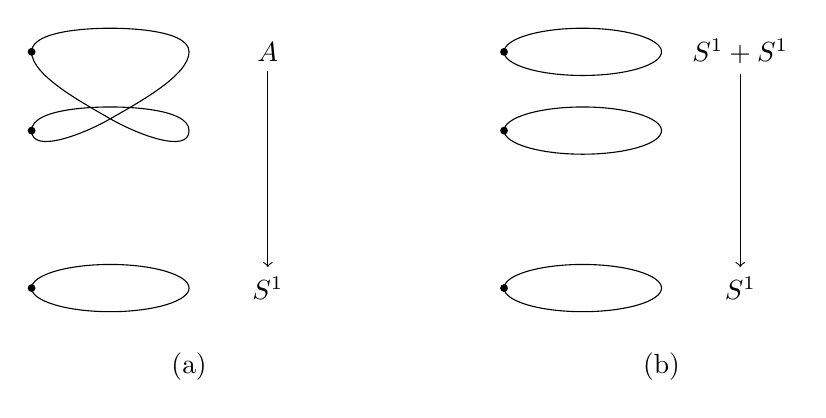
\begin{tikzpicture}
    \node (A) at (2,1) {$A$};
    \node (B) at (2,-2) {$S^1$};
    \draw[->] (A) -- node[auto] {$$} (B);
    \draw (0,-2) ellipse (1 and .3);
    \draw (-1,0)
    .. controls ++( 90:-.3) and ++(210: .4) .. (0,0.15)
    .. controls ++(210:-.4) and ++(270: .3) .. (1,1)
    .. controls ++(270:-.3) and ++(  0: .1) .. (0,1.3)
    .. controls ++(  0:-.1) and ++( 90: .3) .. (-1,1)
    .. controls ++( 90:-.3) and ++(150: .4) .. (0,0.15)
    .. controls ++(150:-.4) and ++(270: .3) .. (1,0)
    .. controls ++(270:-.3) and ++(  0: .1) .. (0,0.3)
    .. controls ++(  0:-.1) and ++( 90: .3) .. (-1,0);
    \node[fill,circle,inner sep=1pt] at (-1,-2) {};
    \node[fill,circle,inner sep=1pt] at (-1,0) {};
    \node[fill,circle,inner sep=1pt] at (-1,1) {};
    \node (L) at (1,-3) {(a)};
    \begin{scope}[xshift=6cm]
    \node (At) at (2,1) {$S^1+S^1$};
    \node (Bt) at (2,-2) {$S^1$};
    \draw[->] (At) -- node[auto] {$$} (Bt);
    \draw (0,-2) ellipse (1 and .3);
    \draw (0,0) ellipse (1 and .3);
    \draw (0,1) ellipse (1 and .3);
    \node[fill,circle,inner sep=1pt] at (-1,-2) {};
    \node[fill,circle,inner sep=1pt] at (-1,0) {};
    \node[fill,circle,inner sep=1pt] at (-1,1) {};
    \node (Lt) at (1,-3) {(b)};
    \end{scope}
  \end{tikzpicture}
  \caption{A visualization of two \coverings over the circle}
  \label{fig:covering}
\end{figure}

\begin{remark}
  It \emph{is} possible to misunderstand what a ``connected \covering'' is: the other interpretation ``all the preimages are connected'' simply would give us an equivalence and is \emph{not} what is intend (equivalences are \coverings, but not necessarily connected \coverings and connected \coverings are not neccesarily equivalences).  

Likewise, for the other qualifications; for instance in a ``finite covering'' $f:A\to B$, the type $A$ is usually \emph{not} a finite set. % ``pointed \covering'' \emph{could} be misunderstood as a function where all the fibers are pointed sets, that is a \covering with a section. 
Also, given a pointed cover, only the preimage over the basepoint comes with a distinguished point; other preimages are merely sets.

  We trust the reader keeps our definitions in mind and not the other interpretations.
\end{remark}
\begin{remark}
  \Coverings are closely related to a concept from topology called ``covering space'' (or any variant thereof, including Galois theory) and from algebra as sheaves (of sets).  Either way, the concept is useful because it singles out the (sub)symmetries.  
% \end{remark}

% \begin{remark}
  \label{rem:setfamloopinj}
  We recall \cref{cor:fib-vs-path} stating that all the fibers of a map $f:A\to B$ are sets if and only if each 
$$\ap{f}: (a=a')\to (f(a)=f(a'))$$ is an injection.
\end{remark}

% \begin{definition}\label{def:decktrafo}\footnote{postpone}
%   Let $f:A\to B$ be a \covering.  A symmetry $(A,f,!)=(A,f,!)$ is called a \emph{deck transformation}.
% \end{definition}
%specified by a pair $(p_A,p_f)$ with consisting of a $p_A:A=_{\UU}A'$, a $p_f:f'p_A=_{A\to B}f$.

\begin{remark}\label{rem:coveringsasfamilies}  
Under the equivalence \cref{lem:Prop-Set-pointed-families}(\ref{lem:Set-families})
between the type $B\to\Set$ of families of sets indexed by $B$, and the type
of \coverings over $B$, we see that we could alternatively have defined a \covering to be a type family $E:B\to\Set$.
%\footnote{it sounds almost cosa nostra to claim that \coverings and families are the same things}  
%In particular, an equivalence (aka.~a family of contractible types) is a \covering.
\end{remark}

We use this point of view straight away:
\begin{example}
  \label{xca:coveringsofS1}
  Let us consider \coverings over the circle, most conveniently for the moment in the guise of families 
$$E:\Sc\to\Set.$$
By the definition of the circle, giving $E$ is the same as specifying a set $E(\base)$ and a symmetry $E(\Sloop):E(\base)=E(\base)$.  Said more concisely in terms of \cref{lem:freeloopspace}, the type of \coverings over the circle is equivalent to 
$$\sum_{X:\Set}(X=X).$$
We will ultimately show that the circle $\Sc$ is equivalent to the component $C$ of $(\zet,s)$ in $\sum_{X:\Set}(X=X)$,  where $s:\zet=\zet$ is the successor.  This may seem sort of circular: ``the circle is equivalent to a component of the type of \coverings over the circle!'' but it really just condenses the idea connected groupoids are uniquely given by their symmetries.
\end{example}
A particularly important example is the following:
\begin{definition}
  \label{def:RtoS1}
  Let the \emph{exponential \covering of the circle}
$$\exp:\mathbb R\to \Sc$$ 
be the \covering of the circle given by $(\zet,s):\sum_{X:\Set}(X=X)$.  
\end{definition}

In more detail, if $R:\Sc\to\Set$ is defined by letting $R(\base)$ be $\zet$ and $R(\Sloop)$ the successor $s$, then 
$$\mathbb R\defequi\sum_{z:\Sc}R(z)$$ 
and $\exp:\mathbb R\to \Sc$ is the first projection.

\begin{remark}
  \label{rem:expforreal}
  The reason for the name $\exp:\mathbb R\to \Sc$ comes from the following visualization.  
%Consider the real and complex numbers $\mathbb R$ and $\mathbb C$.  
If $x$ is a real number, then the complex exponentiation $e^{2\pi i x}=\cos(2\pi x)+i\sin(2\pi x)$ has absolute value $1$ and so defines a continuous function from the real numbers to the unit circle.  
Choosing any point $z$ on the unit circle, we see that the preimage of $z$ under the exponential function is a shifted copy of the integers inside the reals. 
 
This connection between the integers and the unit circle is precisely captured in a form that we can take further by the \covering $\exp:\mathbb R\to \Sc$.
\end{remark}

We already defined a \covering $f:A\to B$ to be universal if $A$ is contractible.  In the situation where $B$ is a pointed groupoid this coincides with the path bundle we have defined more generally.  
Since it is going to be such a central figure, let us repeat the definition and give it the local name.
\begin{definition}
  \label{def:universalcover}
  Let $(B,b_0)$ be a pointed connected groupoid.  
The \emph{universal \covering}\footnote{for $B$ not a groupoid this is total misuse of language.  I feel sort of bad about it, but I did not want to say ``path fibration''} of $B$ is the \covering of $B$ given by the family of sets 
  $$P_{b_0}:B\to\Set,\quad P_{b_0}(b)\defequi (b_0=_Bb),$$
or alternatively as the first projection from $P_{b_0}B\defequi\sum_{b:B}(b_0=_Bb)$ to $B$. 
\end{definition}
Note that $(b_0=_B b)$ is a family of \emph{sets} exactly when $B$ is a groupoid. 
However, we have \cref{lem:thepathspaceiscontractible} for any type $B$.

\begin{remark}
  What's so ``universal'' about this?
  %This seems to deflates the concept ``universal \covering'' of a pointed connected groupoid $(B,b_0)$, since we've just shown that t
The universal \covering over the pointed connected groupoid $(B,b_0)$ coincides with the constant function $c_{b_0}:\bn 1\to B$ (with value $b_0$), and seems like an unnecessary complicated representation were it not for the manifold practical value of the formulation that we've given.  
In particular, we recognize the set of symmetries $b_0=_Bb_0$ as the preimage of $b_0$ under the first projection from $P_{b_0}B$ to $B$; ultimately this will show that the study of symmetries coincides with the study of the universal \covering.

The first instance of this comes already in the next section, where we show in \cref{cor:S1groupoid} that the symmetries of the circle is given by the set of integers $\zet$ by showing that the universal \covering and the exponential \covering (\cref{def:RtoS1}) of the circle coincide.

That said, one way to see that the constant function $c_{b_0}:\bn 1\to B$, \emph{does} deserve the label universal because if given any function $f:A\to B$ and an $(a_0,p): f^{-1}(b_0)$, then we get a function $c_{a_0}:\bn 1\to A$ and $p:b_0=f(a_0)$ gives an element in $c_{b_0}=_{\bn 1\to B}f\, c_{a_0}$.  In other words, any such $f$ is ``a factor of $c_{b_0}$''.  
Note, however, that this depends on $f^{-1}(b_0)$ being non-empty (classically, this is often demanded of a covering, which distinguishes it from our \coverings), and the factorization depends on the element $(a_0,p)$ used. 
\end{remark}




\subsection{The symmetries of the circle}
\label{sec:symcirc}
We now proceed to show that the symmetries $\base=\base$ of the circle is equal to the set $\zet$ of integers.  
The first step is to prove that the exponential \covering \cref{def:RtoS1} is equal to the universal \covering \cref{def:universalcover}, \ie we prove that the family 
$$R: \Sc\to\UU,\qquad R(\base)\defequi\zet,\, R(\Sloop)\coloneq s$$
is equal to the family
$$P_\base:\Sc\to\UU,\qquad P_\base(z)\defequi (\base=z).$$
We define two functions, $f:P_\base\to R$ and $g:R\to P_\base$ and show that, under univalence, they define inverse identities.  

To do this we need to recall from \cref{sec:heavy-transport} how transport behaves in the function type of families.  If given a type $A$ and two type families $P,Q:A\to\UU$, then $(P\to Q)= \prod_{a:A}(P(a)\to Q(a)$.  Then transport along $p:a=_Aa'$ of $f:P(a)\to Q(a)$ is $Q(p)\,f\,P(p)^{-1}:P(a')=Q(a')$, in a picture
$$\xymatrix{
P(a)\ar[r]^{f}\ar@{=}[d]^{P(p)}&Q(a)\ar@{=}[d]^{Q(p)}\\
  P(a')&\,Q(a').}
$$
If $A$ is $\Sc$, then the induction principle for the circle says that giving an $f:P\to Q$ is the same as specifying an $f(\base):P(\base)=Q(\base)$ and an identity $f(\Sloop):Q(\Sloop)\,f(\base)\,P(\Sloop)^{-1}=_{P(\base)\to Q(\base)}f(\base)$, \ie a witness that the composites in 
$$\xymatrix{
  P(\base)\ar[r]^{f(\base)}\ar@{=}[d]^{P(\Sloop)}&Q(\base)\ar@{=}[d]^{Q(\Sloop)}\\
  P(\base)\ar[r]^{f(\base)}&\,Q(\base)}
$$
are equal.  If $P,Q$ are families of sets, then $f(\Sloop)$ is in a proposition.


\begin{definition}
  \label{def:fPtoR}
  The function $f:\prod_{z:\Sc}(P_\base(z)\to R(z))$ is defined by transport: $f(z)(p)\defequi\trp{R,p}0$.\footnote{picture of transport!}
\end{definition}
\begin{definition}
  \label{def:gRtoP}The function $g:\prod_{z:\Sc}(R(z)\to P_\base(z))$ is defined by circle induction: 
$$g(\base)\defequi \Sloop^-:\zet\to(\base=\base)$$ and 
$$g(\Sloop): Q(\Sloop)\, g(\base)\,P(\base)^{-1}=_{Q(\base)\to P_\base(\base)}g(\base)$$ states that if $n:\zet$, then the two elements $Q(\Sloop)\, g(\base)\,P(\base)^{-1}(n)\defequi \Sloop\,\Sloop^{s^{-1}(n)}=\Sloop^{1+n-1}$ and $\Sloop^n$ in $\base=\base$ are equal.
\end{definition}
In a picture, $g(\Sloop)$ demonstrates that starting with $n:\zet$ it does not matter what path you take around the square
$$\xymatrix{\zet\ar[r]^{\Sloop^-}\ar@{=}[d]^s&(\base=\base)\ar@{=}[d]^\Sloop\\
  \zet\ar[r]^{\Sloop^-}&(\base=\base)}
$$




\begin{lemma}
  \label{lem:univisexp}
  The function $f:P_\base\to R$ defined by transport in \cref{def:fPtoR} is an equivalence with inverse $g:R\to P_\base$ defined by circle induction in \cref{def:gRtoP}.  Hence, 
$P_\base$ defines a connected \covering of the circle: $P_\base(z)\defequi (\base=z)$ is a set for all $z:\Sc$ and the type $P_\base \Sc$ is connected (more precisely, by univalence $P_\base(z)$ is equal to the set $R(z)$ and $P_\base \Sc$ is contractible).
\end{lemma}
\begin{proof}
  Firstly we need to give an element $H:g\,f=\id_{P_\base}$, or in other words, that for all $z:\Sc$ and $p:P_\base(z)\defequi(\base=z)$ an element $H(z,p):g(z)\,f(z)(p)=p$.  By the induction principle for the identity type, it is enough to show this for the case $z\oldequiv\base$ and $p\oldequiv\refl\base$ in which case we can set $H(\base,\refl\base)\defequi\refl{\refl\base}$ since
$g(\base)\,f(\base)(\refl\base)\defequi g(\base)(0)\defequi\refl\base$.

Secondly, we need an element $G:g\,f=\id_{R}$, or in other words, that for all $z:\Sc$ and $n:R(z)\defequi\zet$ an element $G(z,p):f(z)\,g(z)(n)=n$.  By circle induction it is enough to provide information for $\base$ and $\Sloop$, but since $\zet$ is a set the information for $\Sloop$ is redundant.  Hence, we need to show that for all $n:\zet$ that $f(\base)\,g(\base)(n)\oldequiv f(\base)(\Sloop^n)$ is equal to $n$.  We do this by induction on $n$.  The case $n=0$ gives $f(\base)(\Sloop^0)\defequi f(\refl\base)\defequi 0$.  For $n=s(m)$ with $m:\NN$ we have\footnote{some references needed here} 
\begin{align*}
  f(\base)(\Sloop^{s(m)})&\defequi\trp{R,\Sloop^{s(m)}}0\\
  &=\trp{R,\Sloop \Sloop^{m}}0\\
  &=\trp{R,\Sloop}(\trp{R,\Sloop^m}0)\\
  &=s(\trp{R,\Sloop^m}0)
\end{align*}
 (the last equality follows since $R(\Sloop)\defequi s$) and by induction on $\NN$ we are done for all positive integers $n$.  For negative $n$ the proof is similar.
\end{proof}


\begin{corollary}\label{cor:S1groupoid}
  The circle $\Sc$ is a groupoid and the function
$$\Sloop^-:\zet\to(\base=_{\Sc}\base)$$ sending $n$ to $\Sloop^n$ is an equivalence.
\end{corollary}
\begin{proof}
  Since the circle is connected, for any $y,z:\Sc$ the type $y=_{\Sc}z$ is equivalent to $base=_{\Sc}z$ which is a set since the function $g(z):\zet\to(\base=z)$ of \cref{def:gRtoP} is an equivalence by \cref{lem:univisexp}.  Hence $\Sc$ is a groupoid, and $g(\base)\defequi\Sloop^-$ is an equivalence.
\end{proof}
\subsection{A reinterpretation of the circle and a criterion for equivalence through \coverings}
\label{sec:S1isC}
In this section we return to the considerations discussed in \cref{xca:coveringsofS1}.
 \footnote{there is duplications here.  Clean it up.}
  Through \cref{lem:freeloopspace} we can get a different perspective on the circle which highlights it as a type classifying very simple symmetries.
By \cref{lem:freeloopspace} (moving up one universe), a type family $\Sc\to\UU$ is uniquely given by a type $X:\UU$ together with a $p:X=_\UU X$, with no further requirements on $p$.  We have seen one example in \cref{def:zet}, namely the one given by the set $\zet$ of integers together with the element $s:\zet=\zet$ given by the successor.  

The importance of this example will become apparent when we eventually explain that \emph{the circle is equivalent to the component $C$ of $\sum_{X:\UU}(X=_{\UU}X)$ containing $(\zet,s)$}. 

Heading towards this goal, we investigate this component a bit further.  Recall from \cref{sec:identity-types} that, in general, if given elements $x,y,z$ in a type $A$, and two identities $f:x=y$ and $g:y=z$, then transport gives rise to the ``composite identity'' $gf:x=z$ (aka $g\circ f$).    Now, if $(X,f):\sum_{X:\UU}(X=_{\UU}X)$, then an element in the identity type $(\zet,s)=(X,f)$ consists of a $p:\zet=X$ and a proof that the succesor $s:\zet=\zet$  is transported along $p$ to $f:X=X$, that is, an element in $psp^{-1}=_{X=X}f$.  Now, by transport, $psp^{-1}=_{X=X}f$ is equivalent to $fp=_{\zet=X}ps$, and so the identity type $(\zet,s)=(X,f)$ is equivalent to
$$\sum_{p:\zet=X}fp=_{\zet=X}ps.$$ % the equation $fp=ps$ comes from the fact that equality in the identity type means that the transport of $s$ along $p$ is equal to $f$, in other words we have an element in $p^{-1}sp=_{X=X}f$ (which we have translated for convenience to an element in $fp=_{\zet=X}ps$).
Since $\zet$ is a set, this identity type is a proposition and so our component $C$ is a connected groupoid.  

In particular, the type of symmetries $(\zet,s)=_C(\zet,s)$ is equivalent to $\sum_{p:\zet=\zet}sp=ps$.  

This discussion tells us that the following definition makes sense:

\begin{definition}\label{def:S1toC}
  Let $C$ be the component of $\sum_{X:\UU}(X=_{\UU}X)$ containing $(\zet,s)$.
  Let $$c:\Sc\to C$$ be defined by $c(\base)\defequi (\zet,s)$ and $c(\Sloop):((\zet,s)=_C(\zet,s))$\footnote{strictly speaking, this $c$ is $\ap c$ -- I have decided not to distinguish between them; ok?} be given by the successor $s:\zet=\zet$ (and $\refl{}:ss=ss$)
\end{definition}

We start by identifying the symmetries of $(\zet,s)$ in $C$:

\begin{lemma}
  \label{lem:IdCisZet}
  Any element in $(\zet,s)=_C(\zet,s)$ is of the form $(s^k,!)$ for some unique $k:\zet$.  In other words,
  the function 
$$\ev_0:((\zet,s)=_C(\zet,s))\to \zet$$ given by $\ev_0(p)=p(0)$ is an equivalence.
\end{lemma}
\begin{proof}
  Given $(p,!):(\zet,s)=_C(\zet,s)$ we must determine $p:\zet=_{\Set}\zet$, which by univalence amounts to giving all the values $p(n)$ for $n:\zet$.  However, since $sp=ps$ we get that $p(n+1)=p(n)+1$ and so induction on $n$ (induction for positive and negative $n$ separately) gives that $p(n)=n+p(0)$.  Hence, $p=s^{p(0)}$ (uniquely since $\zet:\Set$).
\end{proof}

We are going to prove that $c$ is an equivalence.  The method of proof is quite a general and relies or  \cref{lem:eqofconntypes} below, which we will have occasion to return to on several occasions.  In our case the application of  \cref{lem:eqofconntypes} is greatly simplified by the fact that we already know that both $\Sc$ and $C$ are connected groupoids, since then \cref{lem:eqofconntypes} says that it is enough to show that $c$ induces an equivalence from the set of symmetries of $\base$ to the set of symmetries of $(\zet,s)$.\footnote{OLDREMARK: of course, the proof of \cref{cor:S1groupoid} \emph{could} attack $c$ directly, but that would compound the technicalities already present there: at present I prefer splitting it up like this.  I am open for letting the proof of \cref{cor:S1groupoid} be postponed till the end of a chapter, so as not to disrupt the flow of ideas}


\subsubsection{Equivalences and \coverings over connected types}
\label{sec:eqconntypes}

\begin{lemma}
  \label{lem:eqandcovofconntypes}
  Let $X$ and $Y$ be types, $x_0,x_1:X$, let $f:X\to Y$ be a function.  Set $y_0\defequi f(x_0)$ and $y_1\defequi f(x_1)$. Assume given an identity $q:y_0=_Yy_1$. Let 
    $$%f^=_{x_0,x_1}
\ap f:(x_0=_Xx_1)\to (y_0=_Yy_1)$$
be the function of \cref{def:apd} induced by $f$.  Then the  the preimage 
$$(\ap f)^{-1}(q)\oldequiv\sum_{p:x_0=x_1}q=\ap f(p)$$ is equivalent to the identity type 
 $$(x_0,\refl{y_0})=_{f^{-1}(y_0)}(x_1,q).$$ 
If in addition $X$ and $Y$ are connected, then
\begin{enumerate}
\item $f$ is an equivalence if and only $\ap f%f^=_{x_0,x_1}
$ is an equivalence and
\item $f$ is a \covering if and only if  $\ap f%^=_{x_0,x_1}
$ is an injection (\ie if and only if all the preimages of $\ap f$ are propositions).
\end{enumerate}

\end{lemma}
\begin{proof}
((proofread))
  Recall the family $P_{x_0} : X\to\UU$, $P_{x_0}(x)\defequi (x=x_0)$, giving rise to the contractible type $P_{x_0}X=\sum_{x:X}(x_0=x)$.  The function $f$ induces a function of types 
$$P_f:\sum_{x:X}(x_0=x)\to\sum_{y:Y}(y_0=y),\qquad P_f(x,p)=(f(x),\ap f p).$$  Since $P_f$ is a function between contractible types it must be an equivalence.  Hence, the preimage of $(y_0,\refl{y_0})$, 
$$(P_f)^{-1}(y_0,\refl{y_0})\oldequiv\sum_{x:X}\sum_{p:x_0=x}\sum_{r:y_0=f(x)}r=\ap f(p),$$  
is contractible.  
Consider the projection 
$$(P_f)^{-1}(y_0,\refl{y_0})\to f^{-1}(y_0)$$ and observe that the preimage over $(x_1,q:y_0=y_1) $ is equivalent to the preimage $(\ap f)^{-1}(q)\defequi\sum_{p:x_0=x_1}q=\ap f(p)$.  Spelling out the last equivalence: the preimage of $(x_1,q:y_0=y_1) $ spelled out in full is
$$\sum_{x:X}\sum_{p:x_0=x}\sum_{r:y_0=f(x)}r=\ap f(p)\times(\sum_{a:x_1=x}\ap f q=r),$$
which is equivalent to the reshuffle
$$\sum_{p':x_0=x}\sum_{s:q=\ap f p'}\left(\sum_{x:X}(x_0=x)\times\sum_{t:y_0=f(x_1)}(q=s)\right)$$
via the function sending $(x,p,r,u,v)$ to $(a^{-1}p,\ap f a^{-1}\,vu,x,p,\ap f a^{-1}\, r,v)$. ((check))  Now, in the last everything in the parenthesis is contractible, and what is left is exactly $(\ap f)^{-1}(q)$.  Since $(P_f)^{-1}(y_0,\refl{y_0})$ is contractible, this shows that $(\ap f)^{-1}(q)$ is equivalent to $(x_0,\refl{y_0})=_{f^{-1}(y_0)}(x_1,q).$

Now, assume that $X$ and $Y$ are connected.   If $f$ is an equivalence, it follows automatically that the function of identity types is, so we concentrate on the other implication and assume the induced function from $x_0=x_0$ to $f(x_0)=f(x_0)$ is an equivalence.  We want to show that all fibers of $f$ are contractible, but since $Y$ is connected it is enough to consider the fiber $f^{-1}(y_0)\defequi\sum_{x:X}y_0=f(x)$ over $y_0\defequi f(x_0)$.  Now, $(x_0,\refl{y_0})=_{f^{-1}(y_0)}(x_1,q)$ are the fiber of a function from a contractible type to $f^{-1}(y_0)$, so $f^{-1}(y_0)$ is contractible if all the $(x_0,\refl{y_0})=_{f^{-1}(y_0)}(x_1,q)$'s are contractible, which by the previous result is equivalent to $\ap f$ being an equivalence.  

The statement about \coverings is the similar, except that now one desires that the identity types $(x_0,\refl{y_0})=_{f^{-1}(y_0)}(x_1,q)$ should be propositions (for $f^{-1}(y_0)$ to be a set, which then is equivalent to the preimages $(\ap f)^{-1}(q)$ being propositions.
\end{proof}

\begin{lemma}\label{lem:eqofconntypes}\footnote{
%The argument for a general group and the torsors over its abstract group is VERY similar.  
Essentially it is our version of ``a group homomorphism is an isomorphism iff it is a bijection'': proofread}
  Let $X$ and $Y$ be connected types, $x_0:X$ and let $f:X\to Y$ be a function.  Then $f$ is an equivalence if and only if the induced function from $x_0=x_0$ to $f(x_0)=f(x_0)$ is.\footnote{note to self: try to be consistent in writing equalities with right variance (as I hope I have managed to do here)}
\end{lemma}
\begin{proof}
  

 Its fiber over $(y_0,\refl{y_0})$ is 
$$(P_f)^{-1}(y_0,\refl{y_0})\oldequiv\sum_{x:X}\sum_{p:x_0=x}\sum_{q:y_0=f(x)}q=f(p),$$ and is contractible since it is the fiber of a function of contractible types.  
\end{proof}
\begin{lemma}
  Let $X$ and $Y$ be connected types, $x_0:X$ and let $f:X\to Y$ be a function.  Then $f$ is a \covering if and only if the induced function from $x_0=x_0$ to $f(x_0)=f(x_0)$ is an injection.\footnote{embedding/injection...}
\end{lemma}



\begin{theorem}\label{thm:S1bysymmetries}
  The function $c:\Sc\to C$ is an equivalence.
\end{theorem}
\begin{proof}
  In view of \cref{lem:eqofconntypes} we only need to show that the induced function of symmetries $c:(\base=_{\Sc}\base)\to((\zet,s)=_C(\zet,s))$ is an equivalence.\footnote{ ((can we call equivalences between sets bijections?)).}  

The function $\Sloop^-:\zet\to (\base=_{\Sc}\base)$ sending $n:\zet$ to $\Sloop^n$ is an equivalence by  \cref{cor:S1groupoid} and the function  $\ev_0:((\zet,s)=_C(\zet,s))\to \zet$ given by $\ev_0(p)=p(0)$ is an equivalence by \cref{lem:IdCisZet}.  Tracing through the composite function $\ev_0\,c\,\Sloop^-:\zet\to\zet$ we see that $\ev_0\,c\,\Sloop^n=\ev_0\,s^n=n$, (\ie $\ev_0\,c\,\Sloop^-=\id_\zet$) giving that $c$ is an equivalence. 
% The composition with the functions $\Sloop^-:\zet\to (\base=_{\Sc}\base)$ sending $n:\zet$ to $\Sloop^n$ and $\ev_0:((\zet,s)=_C(zet,s))\to \zet$ of \cref{lem:IdCisZet} given by $\ev_0(p)=p(0)$ gives us a function $w:\zet\to\zet$ with $w(n)=s^n(0)$.  From \cref{cor:S1groupoid} we know that $\Sloop^-$ is an equivalence, so we only need to show that $w$ is an equivalence
\footnote{I may have used 2-out-of-3 before, we probably need to include it somewhere, though by univalence it hardly seems necessary}% .  If $p:\zet=\zet$ with $!:sp=ps$, we get by induction on $n:\zet$ (induction for positive and negative $n$ separately) that $p(n)=n+p(0)$.  Hence, all the elements in the preimage $w^{-1}(p,!:sp=ps)$ are equal to $(p(0),!)$.  
\end{proof}

% Now, consider the function 
% $$f:\sum_{p:\zet=\zet}(sp=ps)\to\zet,\qquad f(p,!)=p(0).$$  If $a:\zet$, then $f^{-1}(a)$ consists of the $p:\zet=\zet$ with $sp=ps$ and $p(0)=a$ (the last two are propositions), but by induction we see that $p(n)=n+a$ for all $n:\zet$ (separate induction on positive and negative numbers).  In other words, all elements in the set $f^{-1}(a)$ are equal, and so $f$ is an equivalence


%   ((TODO))
% As an illustration of things to come in a simpler setting, we can give the torsor definition of the circle, where Marc makes the simplifying observation that (since the integers is free on one generator) this can be coded in terms of the successor and there is a priori no need to talk about the abstract group.  In short: an (abstract) $\ZZ$-set is uniquely given by a set $X$ with an identity $f: X=_{\Set}X$.  A $\ZZ$-torsor $(X,f)$ is a $\ZZ$-set (merely) equal to $(\zet,S)$ ($S$ is the successor), that, there is a $p:X=\zet$, so that $Sp=_{X=X} pf$.  This is based at (the pricipal $\ZZ$-torsor represented by) $(\zet,S)$ and $(\zet,S)=(\zet,S)$ consists of $f:\zet=\zet$ s.t. $Sf=fS$.  Such an $f$ must be given by addition by the integer $f(0)$.  This gives us an equivalence between $\Sc$ and the type of (secret) $\ZZ$-torsors.  This will be trivial if we have shown that a map of connected groupoids is an equivalence if it induces an equivalence on the identity sets.

\section{Other \coverings over the circle}
\label{sec:covS1}

\footnote{The below is not fully structured yet, and does contain known nonsense (basepoints, orientations etc need to be straightened out)}
From \cref{lem:eqandcovofconntypes} we know that a function $f:A\to \Sc$ from a connected type $A$ is a \covering if and only if for given $a_0:f^{-1}(\base)$ the induced function from $a_0=_Aa_0$ to $(f(a_0)=f(a_0))=(\base=_{\Sc}\base)$ is injective; or in words, if the symmetries of $a_0$ inject into the symmetries of $\base$ (which by \cref{cor:S1groupoid} may be identified with with the set $\zet$ of integers).

So, a classification of \coverings over the circle amounts to answering the question of what ``subsymmetries'' $\base$ posesses.  Using language yet to be introduced, the question would be ``what are the subgroups of the integers?''

\begin{example}
  \label{ex:listofS1covers}
  \begin{enumerate}
  \item The \emph{universal} \covering  $$c_\base:\bn 1\to \Sc$$ sends the unique element of $\bn 1$ to $\base$ is a \covering. The universal \covering corresponds to the trivial subsymmetry of $\base$ (\ie including only $\refl\base$).  
  \item If $m:\NN$ is positive, consider the \emph{degree $m$ function} $$-^m:\Sc\to \Sc$$ given by $-^m(\base)\defequi\base$ and $-^m(\Sloop)\defequi\Sloop^m$.  On the level of identity types and under the equivalence $\Sloop^-:\zet\simeq(\base=_{\Sc}\base)$, this \covering corresponds to the function $\zet\to\zet$ given by multiplication by $m$.  Hence, the subsymmetries in determined by the degree $m$ function are correspond to the integers divisible by $m$.
  \end{enumerate}
  In the course of our discussion, we will see that -- under an assumption on the setup called ``LPO'', c.f. \cref{LPO} -- these are all the connected decidable \coverings over the circle.
\end{example}

\begin{remark}
  \label{rem:RtoS1}
  The first case, namely the manifestation of the contractible type as a \covering of the circle is important in many applications.  Classically it corresponds to the trigonometric functions sending the real number $x$ (the real numbers form a contractible space) to the point $(\cos x,\sin x)$ on the unit circle in the plane.  If you're familiar with complex numbers, you may want to say that this \covering is the exponential function sending the real number $x$ to the point $e^{2\pi ix}$ on the unit circle in the complex plane.

  \label{rem:finitecoveringsofS1}
  The analogue of our degree $m$ function is the $m$th power of complex numbers restricted to the unit circle.  The following is perhaps more tangible.  Let $m=12$ and picture the circle and mark $12$ evenly spaced points.  This will look like a clock, with marks $1,2,\dots,12$.  You can then make a function from the circle to itself by sending all marks to $12$ and each of the arcs connecting the marks to the entire circle -- (in a continuous manner preserving the orientation).
  ((picture!!))
\end{remark}

We could be more ambitious and ask: what is the \emph{type} of decidable \coverings over the circle?  Since the type of \coverings is equivalent to $\Sc\to \Set$, and the fact that if $F,F':\Sc\to\Set$, then $F=_{\Sc\to\Set}F$ is the type $\prod_{z:\Sc}(F(z)=_{\Set}F'(z))$ (which is a set\footnote{reference}), we see that the type of decidable \coverings over the circle is a groupoid.  We will pin this groupoid down by first identifying the components (of which there turns out to be one for each natural number), and then analyzing one component at a time.

 Recall the function $c:\Sc\to C$ of \cref{def:S1toC}.  By \cref{thm:S1bysymmetries} we know that $c$ is an equivalence, so classifying \coverings over $\Sc$ is equivalent to classifying \coverings over $C$.  
We simplify the notation slightly, letting $\pt_C\defequi(\zet,s):C$ (the element corresponding by \cref{def:S1toC} to $\base:\Sc$), and allowing ourselves to write $s:\pt_C=_C\pt_C$ instead of the more honest $(s,!):\pt_C=_C\pt_C$ (corresponding to $\Sloop:\base=\base$).

 Returning to \cref{ex:listofS1covers}, it is instructive to rephraze these connected \coverings in terms of $C$.
\begin{example}
 \label{ex:listofCcovers}\label{ex:Cunivcov}
The universal connected \covering is still represented by the constant function
    $$c_{(\zet,s)}:\bn 1\to C$$ that sends the unique element of $\bn 1$ to $(\zet,s):C$.
    \end{example}
    \begin{example}
      \label{ex:mfoldcov}
Assume that $m:\NN$ is positive.  We give a description of the $m$-fold \covering of the circle in terms of $C$. If $X$ is a set and $f:X\to X$ we define the \emph{ $m$th root}
$$\sqrt[m]f:\bn m\times X\to\bn m\times X$$ by setting 
$$\sqrt[m]f(i,x)=
\begin{cases}
  (i+1,x)& \text{for $i<m-1$ and}\\(0,f(x))& \text{for $i=m-1$}.\footnote{this indexing uses the incarnation $\bn m=\{0,1,\dots m-1\}$ and not $\{1,\dots,m\}$: if this is a problem we should change $\bn m$ since the indexing chosen is very convenient later.}
\end{cases}$$ 
Only one $m$th of the time does $\sqrt[m]f$ use $f$ on $X$ (the rest of the time it increases the element in $\bn m$).  This is illustrated in \cref{fig:root} with the shift by $f$ being vertical and the movement along $\bn m$ going around a circle.  
\begin{figure}
  \centering
  \begin{tikzpicture}
    \node (A) at (4,1) {\quad$\sqrt[m]f:\bn m\times X\to\bn m\times X$};
    \foreach \y in {0,1,2}
    { \begin{scope}[shift={(0,\y)}]
        \foreach \x in {0,...,4}
        { \node[fill,circle,inner sep=1pt] at (180+72*\x:1 and .3) {}; }
        \foreach \x in {0,...,3}
        { \draw[-stealth] (180+72*\x:1 and .3) arc(180+72*\x:252+72*\x:1 and .3); }
      \end{scope} }
    \foreach \y in {1,2}
    { \begin{scope}[shift={(0,\y)}]
        \draw[-stealth] (108:1 and .3)
        .. controls ++( 5:-.3) and ++(80:.2) .. (-.7,-.4)
        .. controls ++(80:-.2) and ++(90:.2) .. (-1,-1);
      \end{scope} }
    \draw[-stealth] (108:1 and .3)
    .. controls ++( 5:-.3) and ++(80:.2) .. (-.7,-.4);
    \node (dz) at (-.7,-.7) {\footnotesize$\vdots$};
    \begin{scope}[shift={(0,3)}]
      \draw[-stealth] (-.7,-.4)
      .. controls ++(80:-.2) and ++(90:.2) .. (-1,-1);
      \node (da) at (-.7,0) {\footnotesize$\vdots$};
    \end{scope}
    \draw [decorate,decoration={brace,amplitude=10pt}]
    (-1.1,-.8) -- (-1.1,2.8) node [black,midway,xshift=-20pt] {\footnotesize $X$};
    \draw [decorate,decoration={brace,amplitude=10pt}]
    (1,-1) -- (-1,-1) node [black,midway,yshift=-15pt] {\footnotesize $\bn{m}$};
  \end{tikzpicture}
  \caption{The $m$'th root of an endomorphism}
  \label{fig:root}
\end{figure}
Indeed, iterating $\sqrt[m]f$ we get $(\sqrt[m]f)^m(i,x)=(i,f(x))$; hence the term ``$m$th root'' is apt.

If $f$ is an equivalence, then so is $\sqrt[m]f$:
\begin{enumerate}
\item on one hand $(\sqrt[m]f)(j,y)$ is equal to $(0,x)$ if and only if $j=m-1$ and $f(y)=x$, so  $(\sqrt[m]f)^{-1}(0,x)$ is equivalent to $f^{-1}(x)$ which is contractible if $f$ is an equivalence, and 
\item on the other, if $i:\bn m$ is not $0$, then $(\sqrt[m]f)(j,y)$ is equal to $(i,x)$ if and only $j+1=i$ and and $y=x$, and so  $(\sqrt[m]f)^{-1}(i,x)$ is equivalent to  a singleton.
\end{enumerate}


Using univalence, the $m$th root construction applies not only to equivalences, but equally well to identities $f:X=_{\Set}X$; resulting in a function 
$$-^m:\sum_{X:\Set}(X=X)\to\sum_{X:\Set}(X=X),\quad -^m((X,f))=(\bn m\times X,\sqrt[m]f).$$
We now focus on  $C$, the component of $\sum_{X:\Set}(X=X)$ containing $(\zet,s)$.
Note that the function $p:\bn m\times \zet\to\zet$ given by $p(i,n)=i+mn$ is an equivalence and that 
$$p\sqrt[m]s(i,n)=i+1+mn=sp(i,n).$$  
Consequently $(\bn m\times\zet,\sqrt[m]s):\sum_{X:\Set}X=_\UU X$ is in the component of $(\zet,s)$, \ie $(\bn m\times \zet,\sqrt[m]s):C$.\footnote{\color{red} Note to self: Marc wants to expand on this (hand written note)} % In consequence, if $(X,f):C$ (\ie $(X,f):\sum_{X:\Set}X=_\UU X$ is in the component of $(\zet,s)$) then also $(\sqrt[m]X,\sqrt[m]f):C$, giving rise to the 
Ultimately, we have defined the
 \emph{degree $m$ function} $$-^m:C\to C,\qquad -^m((X,f))=(\bn m\times X,\sqrt[m]f).$$
% , where $$\sqrt[m]X=\bn m\times X$$ and $\sqrt[m]f(i,x)=(i+1,x)$ for $i<m-1$ and $\sqrt[m]f(m-1,x)=(1,f(x))$.  We prove that $-^m((X,f))$ is in the component of $(\zet,s)$ (which was a requirement for elements in $C$).
 % Since we know that $(X,f)$ is in the component of $(\zet,s)$ it is enough consider the element $(p,!):(\sqrt[m]{\zet},\sqrt[m]s)=(zet,s)$ explicitly given by univalence through $p((i,n))=i+mn$ ((check that it gives an equivalence)).

If $(p,!):(X,f)=_C(X',f')$, then 
$$(\id\times p,!):(\bn m\times X,\sqrt[m]f)=(\bn m\times X',\sqrt[m]f')$$ 
is given by % $(\id\times p)(i,x)=(i,p(x))$ (and by 
the fact $!:(\id\times p)\sqrt[m]f=_{\bn m\times X=\bn m\times X'}\sqrt[m]{f'}(\id\times p)$\footnote{$(i,x)$ is taken to $(i+1,px)$ if $i<m-1$ and $(m-1,x)$ is taken to either $(0,f'px)$ or $(1,pfx)$ which are equal by assumption}.  In particular, letting $p\defequi s:\zet=\zet$, we get that $(\id\times s)(i,n)=(i,sn)=(\sqrt[m]s)^m(i,n)$.

This will eventually ((forwardref)) be explained in terms of the symmetries of the degree $m$ \covering of the circle being given by the powers of $\sqrt[m]s$ in a nonunique fashion: 
for any $a:\zet$, the $a$th and the $(a+m)$th power of $\sqrt[m]s$ give rise to the same symmetry.


Why does this correspond to the $m$-fold \covering we defined in \cref{ex:listofS1covers}?  This is ecapsuled by the fact that under the equivalence $c:\Sc\to C$ the two $m$-fold covers agree in the sense that the two functions given as composites in
$$\xymatrix{\Sc\ar[r]^c\ar[d]^{-^m}&C\ar[d]^{-^m}\\\Sc\ar[r]^c&C}$$ are equal.  One composite is given by $-^mc(\base)=(\zet,s)$ and $-^mc(\Sloop)=s^m$ and the other is given by $c-^m(\base)=(\bn m\times\zet,\sqrt[m]s)$ and $c-^m(\Sloop)=\id\times s$ and the proof that these two functions are equal is given by the (identity corresponding by univalence to the) equivalence  $p:\bn m\times \zet\to\zet$ with $p(i,n)=i+mn$ we discussed above, since transport of $\sqrt[m]s$ along $p$ is exactly $s^m$ (\ie $p\sqrt[m]s=s^mp$: note the way we formulate this so that we don't need to talk about an inverse of $p$).
\end{example}
\begin{xca}
  Check the implicit claims in \cref{ex:listofCcovers}.  ((perhaps best to make them explicit?))
\end{xca}
There are many instance of the $m$-th root construction which is of independent interest.  We record the following for future reference.
\begin{definition}
  \label{def:Zetmodm}
  Let $m$ be a positive integer.
  The element $\zet/m:\sum_{X:\Set}(X=X)$ has first projection $\bn m\times\bn 1$ and second projection $\sqrt[m]{\id}$.
\end{definition}
This realizes the cycle $0\mapsto1\mapsto\dots\mapsto m-1\mapsto 0$ in $\bn m$, and so models ``modular arithmetic''.


Any (other) textbook will tell you that these are all the connected \coverings over the circle (precisely one for each natural number), but the procedure is unfortunately not constructive: we need a further assumption which is not generally present in our setup, namely

\begin{quote}
  {\bf The Limited Principle of Omniscience} (LPO)\index{LPO}\label{LPO}\footnote{make an environment that principles can fit in and be numbered} If given a function $P:\NN\to\bn 2$, then either $P$ is constant (we have that $\prod_{n:\NN}(P(0)=P(n))$) or there is an $n_0:\NN$ such that $P(n_0)\neq P(0)$.
\end{quote}
LPO is weaker than the law of excluded middle and we are free to assume it as an axiom -- or not.  We will be explicit about where we will use it.


Fix for the moment a connected type $A$ and a decidable \covering 
$$f:A\to C$$ (c.f \cref{def:covering}) and an element $\pt_A:f^{-1}(\pt_C)$.  %Assume $(\pt_A,!):f^{-1}(\pt_C)$
%Recall the element 
%$$\pt_C\defequi(s,\refl{ss}):(\zet,s)=_C(\zet,s),$$ which by \cref{def:S1toC} corresponds to $\Sloop:\base=\base$.
By \cref{lem:eqandcovofconntypes}, the fact that $f$ is a decidable \covering exactly says that the induced function of identity types
$$g\defequi\ev_0f^=:(\pt_A=_A\pt_A)\to (\pt_C=_C\pt_C)=\zet$$ is 
injective and (the fibers are) decidable.\footnote{say this in a way consistent with the choices of subsets/injections/embeddings}    

Assume LPO.  We are then left with two situations (use that $g$ is injective and decidable): either $\pt_A=_A\pt_A$ is contractible or there is a $p_0:\pt_A=_A\pt_A$ with $g(p_0)$ different from $0$. 

In the former case ($\pt_A=\pt_A$ is contractible), \cref{lem:eqandcovofconntypes} together with the fact that $A$ is connected implies that $A$ itself is contractible.  

On the other hand, if $p_0:\pt_A=\pt_A$ with $g(p_0)$ different from $0$, then either $g(p_0)$ or $g(p_0^{-1})$ is a positive integer.  Hence the set $H^+$ of positive integers in the image of $g$ is nonempty, and so the fact \cref{def:Nwellordered} that $\NN$ is well ordered implies that $H^+$ has a minimum, \ie there is a $p:\pt_A=\pt_A$ with  $g(p)=m\defequi\min H^+:H^+$.  Furthermore, if $q:\pt_A=\pt_A$ is any element with $0<g(q)$, then  by Euclidean division of \cref{lem:euclid-div}, there exist $k,r:\NN$ with $r<m$ so that $g(q)=km+r$.  Now, the natural number $r$ is in the image of $g$ (because $r=g(q)-km=g(qp^{-k})$) and is less than the minimal positive value $m=g(p)$, and so we must conclude that $r=0$, or in other words, $g(q)$ is a multiple $g(p)k$ of the minimal positive value $g(p)$.

% \cref{cor:arch} there is a $k:\NN$ such that $g(p)k\leq g(q)<g(p)(k+1)$, or equivalently $0\leq g(q)-g(p)k< g(p)$.  Since $g(q)-g(p)k=g(qp^{-k})$ is a nonnegative integer is in the image of $g$ and simultaneously less than the minimum positive value $g(p)$, we must conclude that $g(q)=g(p)k$.\footnote{rewrite/simplify given that Euclid is now in intro}

Arguing similarly for the negative values, we reach the conclusion that the image of $g$ in $\zet$ is the subset of multiples of $g(p)=\min H^+$.  Hence, the image of $f^=:(\pt_A=\pt_A)\to(\base=_{\Sc}\base)$ is uniquely given by the positive integer $\min H^+$, and is not dependent on $\pt_A$.\footnote{how to say this gently without starting to much fuss regarding commutativity?}  Furthermore, if $p_A:A=_{\UU}A'$, $f':A'\to B$ and $p_f:f'p_A=_{A\to B}f$, then tracing through the argument, we see that the positive number reached through arguing with $f':A'\to B$ remains the same, but there \emph{is} a possibility that $g(p_0)$ changes sign, so that the minimum of $H^+$ is now not attained by $g(p_0)$, but by $g(p_0^{-1})$.\footnote{maybe some HoTT guy can say this less classically.  We also want to say something about the connection to pointed \coverings, conjugations etc to clear the path for later applications}

\begin{lemma}
  \label{lem:componentsofcoversofS1}
  % Assume the LPO. Given a connected decidable \covering of the circle,  there is a unique natural number $m$ so that the connected \covering is equal to the connected \covering $-^m$ of \cref{ex:listofS1covers}.  This gives an equivalence between $\NN$ and the propositional truncation of the type of connected decidable \covering of the circle.
  \begin{enumerate}
  \item The type of decidable \coverings over the circle by connected types is a groupoid.
  \item Assuming, the LPO the type of decidable \coverings over the circle by connected types is the sum of the component containing the universal \covering and for each positive integer $m$, the component containing the $m$-fold \covering.
  \end{enumerate}

\end{lemma}


% A natural question is, given $m:\NN$, what does the associated connective \covering $f:A\to \Sc$ look like?

% We saw that if $m=0$, then the identity types of $A$ were contractible, and so (in view of \cref{lem:eqandcovofconntypes} since $A$ is connected) $A$ is itself contractible.

\begin{remark}
  \label{rem:flipthecircle}
  The reader may wonder how the ``orientation reversing'' $c:\Sc\to \Sc$ given by $c(\base)=\base$ and $c(\Sloop)=\Sloop^{-1}$ fits into the picture.  In our setting it is equal to the identity on $\Sc$ (corresponding to $m=1$): Letting also $c:\Sc=\Sc$ be the identity given by univalence, we have that $\refl{\Sc}=c\cdot c$, so that $c$ itself proves that $\id_{\Sc}$ and $c$ are equal.
\end{remark}

\section{Symmetries of \coverings of the circle are ``cyclic'' }
\label{sec:deckS1}

% In this section we prove the following result.  
The term ``cyclic'' in the chapter heading refers to the fact that we show that the symmetries of \coverings are determined by iterations of a single symmetry.  



\begin{remark}
Since we are interested in the symmetries of particular \coverings it is good to spell out some details.
By \cref{lem:isEq-pair=} (DAN WILL CHECK THIS) the identity type  
$(A,f,!)=(A',f',!)$ of two \coverings over the type $B$ is equivalent to 
\[
\sum_{p_A:A=_{\UU}A'}(f'p_A=_{A\to B}f). 
\]
$$\xymatrix{A\ar@{=}[rr]^{p_A}_\to\ar[dr]_f&&A\ar[dl]^{f'}\\&\,B.&}$$
Here and below, the $p_A$ in the equation $f'p_A=_{A\to B}f$ is 
shorthand for the canonical equivalence from $A$ to $A'$ 
coming from the identification $p_A:A=_{\UU}A'$ by first
applying $\cast:(A=A')\to (A\equiv A')$, and then
applying $\fst:(A\equiv A')\to(A\to A')$ to the result,
in total $\fst(\cast(p_A)): A\to A'$.
\end{remark}

\begin{theorem}
  \label{thm:coveringsofS1}
  \begin{enumerate}
  \item 
  The set $c_\base=c_\base$ of symmetries of the universal \covering of the circle is equivalent to $\zet$.  
Furthermore, there is a symmetry $$Q^1:c_\base=c_\base$$ so that, considered as an element in $\sum_{X:\Set}X=X$ the pair $(c_\base=c_\base,Q^1)$ is equal to $(\zet,s)$.  

The component of the type of \coverings over the circle containing the universal \covering is equivalent to the circle via the map from $S^1$ sending $\base$ to $c_\base$ and $\Sloop$ to $Q^1$.
\item For a positive integer $m$, the set $-^m=-^m$ of symmetries of the $m$-fold \covering of the circle is equivalent to $\bn m$.  

Furthermore, there is a symmetry $$Q^1:-^m=-^m$$ so that considered as an element in $\sum_{X:\Set}X=X$ the pair $(-^m=-^m,Q^1)$ is equal to $\zet/m$ of \cref{def:Zetmodm}.

The component of the type of \coverings over the circle containing the $m$-fold covering is equivalent to $$\sum_{X:\Set}\sum_{p:X=X}||(X,p)=\zet/m||.$$
  \end{enumerate}

 \end{theorem}
\begin{remark}\label{rem:thenonuniquenessofgeneratorsofmodulararithmetic1}
  The symmetries called $Q^1$ in \cref{thm:coveringsofS1} are not uniquely determined by the stated property.  
In the case of the universal \covering there are two candidates and for the $m$-fold \covering there are as many as there are positive integers less than $m$ that does not divide $m$.  
This behavior has number theoretic consequences and origins and will be investigated further when we have the proper machinery to put it to good use.
\end{remark}

  \begin{proof}
  ((spell out $Q^1$))
We are going to investigate the set 
$$D_0\defequi\sum_{g:\bn 1=\bn 1}c_\bullet g=c_\bullet$$ 
of symmetries of the universal \covering $c_\bullet$ of the circle.  
Our preferred interpretation of $c_\bullet:\bn 1\to C$ is as the first projection from $P\defequi\sum_{(Y,g):C}(\zet,s)=(Y,g)$ to $C$, and the equivalence $c_{((\zet,s),\refl{})}:\bn 1\to P$. % sends the unique point in $\bn 1$ to $(\zet,s):C$ and $\refl{}:(\zet,s)=(\zet,s)$. 
More generally, for any type $A$ the function $A\to(\bn 1\to A)$ sending $a:A$ to the function $c_a$ sending the unique element in $\bn 1$ to $a$ is an equivalence, and if $A$ is contractible, then every $c_a$ is an equivalence.

   Consequently, $D_0$ is equivalent to
$$\sum_{((Y,g),p):P}(\zet,s)=_C(Y,g)$$ 
which can be rewritten as
$$\sum_{(Y,g):C}((\zet,s)=_C(Y,g))\times((\zet,s)=_C(Y,g))
$$
For any $a,b:A$ the ``shear'' 
$$\mathrm{shear}:((a=_Ab)\times(a=_Ab))\to((a=_Ab)\times(a=_Aa))$$ 
given by $\mathrm{shear}(p,q)\defequi(p,q^{-1}p)$
is an equivalence and
% The function in 
% $((\zet,s)=_C(Y,g))\times(((\zet,s)=_C(Y,g))\to (((\zet,s)=_C(Y,g)\times(\zet,s)=_C(\zet,s))$ sending $(p,q)$ to $(p,q^{-1}p)$ is an equivalence,
so $D_0$ is equivalent to 
$$\sum_{(Y,g):C}((\zet,s)=_C(Y,g))\times ((\zet,s)=_C(\zet,s)).
$$
Using the equivalence $\ev_0:((\zet,s)=_C(\zet,s))\equiv\zet$ of \cref{lem:IdCisZet}, this
 reduces to 
$$D_0\simeq P\times\zet\simeq\zet.$$
    
((this does most of what is needed for the $m$-fold \covering.  Needs to be proofread))
    Let $m$ be a positive integer.  
Recall the $m$-fold \covering, either in the guise $-^m:\Sc\to \Sc$ of \cref{ex:listofS1covers} or $-^m:C\to C$ of \cref{ex:listofCcovers}.
We are going to investigate the set
$$D_m\defequi\sum_{g:\Sc=\Sc}-^mg=_{\Sc\to \Sc}-^m$$  
%$$D_m\defequi\sum_{g:C=C}-^mg=_{C\to C}-^m$$ 
of symmetries of the $m$-fold \covering of the circle% , or equivalently, by univalence, $\sum_{t:C\simeq C}-^mt=_{C\to C}-^m$
.  
By univalence and thanks to the equivalence $c:\Sc\to C$ of \cref{thm:S1bysymmetries} $(\Sc= \Sc)$ is equivalent to $(\Sc\simeq C)$.
Since being contractible is a proposition, $\Sc\simeq C$ is a subtype of $\Sc\to C$,
% Thanks to the equivalence $c:\Sc\to C$ of \cref{thm:S1bysymmetries} $(C\to C)$ is equivalent to $(\Sc\to C)$,
which by \cref{lem:freeloopspace} is ultimately equivalent to $\sum_{(Y,g,!):C}(Y,g,!)=(Y,g,!)$. 
For the moment we'll investigate the simpler type 
$$F_m\defequi\sum_{t:\Sc\to C}-^mt=_{\Sc\to C}-^mc$$
and on the way discover that if $(t,Q):F_m$, then $t$ is an equivalence, so that $F_m$ actually {\bf is} equivalent to the type $D_m$ we are interested in.

Given If $t:\Sc\to C$ is given by $t(\base)\defequi (Y,g,!)$ (where $!$ asserts that $(Y,g)$ lies in the component of $(\zet,s)$)  and $t(\Sloop)=(p,!,!):(Y,g,!)=_C(Y,g,!)$, (where $p:Y=Y$ and $pg=gp$ (an identity in the set $Y=Y$)), we study the type $-^mt=_{\Sc\to C}-^mc$.
Spelling out the details we see that $-^mc$ is defined by 
$$-^mc(\base)=(\bn m\times\zet,\sqrt[m]s,!)$$ and 
$$-^mc(\Sloop)\defequi(\id\times s,!,!):(\bn m\times\zet,\sqrt[m]s,!)=_C(\bn m\times\zet,\sqrt[m]s,!)$$   and $-^mt$ is given by $$-^mt(\base)\oldequiv(\bn m\times Y,\sqrt[m]g,!)$$ and 
$$-^mt(\Sloop)\oldequiv(\id\times p,!,!):(\bn m\times Y,\sqrt[m]g,!)=_C(\bn m\times Y,\sqrt[m]g,!).$$

An element in $Q:-^mc=-^mt$ is then given by a 
$$q:\bn m\times\zet=\bn m\times Y$$ so that $\sqrt[m]g\ q=q\sqrt[m]s$ and $q(\id\times s)=(\id\times p)q$ (both in $\bn m\times\zet=\bn m\times Y$). 
Now, the element $$q^{-1}(\id\times s)q=q^{-1}(\sqrt[m]s)^mq=(q^{-1}\sqrt[m]sq)^m$$ in $\bn m\times Y=\bn m\times Y$ is both equal to $\id\times p$ and equal to $(\sqrt[m]g)^m=\id\times g$, proving that $p=g$. 


Consider another element $(t',Q'):F_m$ (as for $(t,Q)$, we spell out $(t',Q')$ in terms of its accompanying $Y'$, $g'$ and $q'$). 
An identity  $R:(t,Q)=_{F_m}(t',Q')$ consists of a $\rho:t=t'$ and an $s:(-^m\rho)Q=_{-^mc=-^mt'}Q'$ (note that this is a proposition), \ie $R$ is given by an $r:Y=Y'$ with 
$$g'r=_{Y=Y'}rg\text{ and }(\id\times r)q=_{\bn m\times Y=\bn m\times Y'}q'(\id\times r).$$  This shows that every $(t,Q):F_m$ is equal to one with $(Y,g)$ being $(\zet,s)$ and $p$ being $s$, and we \emph{could} reduce to this case, leaving to $q$ the entire burden of proof.  
This also shows another thing: the $t:\Sc\to C$ fitting in pairs $(t,Q):F_m$ are all equivalences, so that $F_m$ actually is equivalent to the type $\sum_{g:C=C}-^mg=_{C\to C}-^m$ we are trying to understand.

 On the level of equivalences $\zet\simeq Y$, the equation  $\sqrt[m]g\ q=q\sqrt[m]s$ claims that providing $q$ is the same as providing a point $q(0,0):Y$ through the equation  
$$q(i,n)=q((\sqrt[m]s)^{i+nm}(0,0))=(\sqrt[m]g)^{i+nm}q(0,0).$$  For $(i,k)\in \bn m\times\zet$ define $Q^{(i,k)}$ by setting its first projection to be $q^{(i,k)}=(\sqrt[m]g)^{i+km}q$.  
This exhausts all possible $q(0,0):Y$, so we have accounted for all possible $Q$s.

However, there is some redundancy: since $(\sqrt[m]g)^{i+km}=(\sqrt[m]g)^i(\id\times g^k)$, we have that $g^k:Y=Y$ proves that $Q^{i+km}=Q^{i}$.  ((explain why there is no more redundancy)) 

In hindsight we can give concrete descriptions of all the symmetries: for $i=0,\dots m-1$, let $(Y,g)\defequi (\zet,s)$, $p\defequi s$, and $q(0,0)\defequi i$.

With respect to the identification of the component of the $m$-fold covering.  The type of coverings of the circle is equivalent to $\sum_{X:\Set}X=X$ and by the above, the \covering being in the component of the $m$-fold cover corresponds to $(X,p)$ being in the component of $\zet/m$.
  \end{proof}

  \begin{remark}
    Regarding the symmetries of the $m$-fold \covering of the circle, recall the picture we tried to evoke in \cref{rem:finitecoveringsofS1}.  How can I move my circle with $m$ evenly spaced marked points  (which we now call $0,1,\dots, m-1$ instead of $1,2,\dots 12$ since it fits better with future applications) without disturbing the projection down to the circle (sending all the marked points to $0$).  I can move the marked points, but a marked point has to be sent to a marked point (otherwise the projection down to the circle would be disturbed).  Let's say that mark $0$ is sent to mark $4$.  However, since we have to preserve the projection down to the circle, the arc from $0$ to $1$ must then be sent to the arc from $4$ to $5$.  Continuing in this fashion, we see that we describe a certain rotation of the circle.  Varying $4$ between $0$ and $m-1$ we see that there are exactly $m$ different symmetries of the $m$-fold \covering.  Furthemore they are all rotations of the circle by an angle which is a multiple of $2\pi/m$.
  \end{remark}


{\color{blue}\small\section{desiderata}\footnote{the exercises/definitions of this section should go in a previous chapter}
The following definitions/exercises/notations/etc is used freely, but should probably be elsewhere.

\subsection{Request wrt notation}
\label{sec:requestnotation}

If $f:A\to B$ and $(a,p):f^{-1}(b)$ (for $a:A$, $b:B$ and $p:f(a)=b$), then the function
$$\mathrm{ad}_p\ap f:(a=a)\to(b=b)$$
needs a simpler name.  
I have occasionally sinned and called it $f^=$ (with $p$ implicit).  
I am now converging to using ``$f^p$'' (superscript since I have needed it in situations with other subscripts).


\subsection{Negative numbers}
This is to be deleted when integers are stable
%\label{sec:negativenumbers}


\begin{definition}
  %\label{def:zet}
\footnote{To the one who ports: I \emph{would} have preferred to define $\zet$ as a set quotient of $\NN\times\NN$, but I hoped we could avoid the book discussion (257).  A price is paid when defining the successor.  Given the disclaimer following the formal definition, it is safe to change the definition if you like}
  The \emph{set of integers} is the set
$$\zet\defequi \sum_{(m,n):\NN\times\NN}(r(m,n)=_{\NN\times\NN}(m,n)),$$
where $r:\NN\times\NN\to\NN\times\NN$ is given by
$$r(m,n)\defequi
\begin{cases}
  (m-n,0)&\text{if $m\geq n$}\\
  (0,n-m)&\text{otherwise.}
\end{cases}
$$
We define the \emph{standard inclusion} 
$$i:\NN\to\zet$$ by $i(m)=((m,0)\refl {(m,0)})$ (makes sense since $r(m,0)\defequi(m,0)$), the \emph{negative inclusion} $-:\NN\to\zet$ by $-n=((0,n),\refl{(0,n)})$ and the quotient $q:\NN\times\NN\to\zet$ by $q(m,n)=(r(m,n),\refl{r(m,n)})$ (makes sense since $r(r(m,n))\oldequiv r(m,n)$).  

The successor $s:\zet=\zet$ is defined through univalence from $S : \NN\times\NN\to\NN\times\NN$ with $S(i(n))=i(S(n))$  and $S(-(Sn))=-n$ for $n:\NN$ (check that $S$ is an equivalence: ``any integer is the successor of exactly one integer'').
\end{definition}

Not wishing to mystify things more than necessary, we will refer to $i(n):\zet$ for $n:\NN$ as ``$n:\zet$'', so that any element of $\zet$ is ``plus or minus a natural number'', dividing the non-zero integers into the positive and negative integers.  We extend the order relation by saying that positive integers are greater than negative integes and by saying that $-m\leq -n$ if $n\leq m$ for $m,n:\NN$.
}%endfootnote (Negative integers)

% \subsubsection{Equivalences}
% \label{sec:equivalences}
% Two types are equivalent if you can freely translate back and forth between them: 
% \begin{definition}
%   Let $A$ and $B$ be types.  The type of \emph{equivalences} from $A$ to $B$ is
% $$\Eq(A,B)\defequi\sum_{f: A\to B}\left(\sum_{g:B\to A}\prod_{a:A}g(f(a))=a\right)\times\left(\sum_{h:B\to A}\prod_{b:B}f(h(b))=b\right).
% $$
% \end{definition}
% \begin{remark}
%   You recognize the spirit of ``inverse function'' in the definition of equivalences: an equivalence is a function $f:A\to B$ which has a $g:B\to A$ so that for all $a:A$ we have $g(f(a))=a$ and also an $h:B\to A$ so that for all $b:B$ we have that $f(h(b))=b$.  We will see in Lemma~\ref{lem:leftinvisrightinv} that this forces $g$ and $h$ to be equal, but it is technically convenient not to insist on this in the definition itself.  We refer to $g$ as a \emph{left inverse} of $f$ and $h$ as a \emph{right inverse} of $f$.
% \end{remark}


% \begin{lemma}
%   Given $f : A\to B$, the type of left inverses of $f$, 
% $$\sum_{g:B\to A}\prod_{a:A}g(f(a))=a,$$ is a proposition.  Consequently, the projection $\Eq(A,B)\to (A\to B)$ is a monomorphism.
% \end{lemma}
% \begin{proof}
%   ((write)) 4.2.9
% \end{proof}
% \begin{remark}
%   In view of this result, we will say that $f:A\to B$ \emph{is an equivalence from $A$ to $B$} if it is the projection of an equivalence from $A$ to $B$.  Occasionally the following alternative notation is more convenient:
% $$(A\simeq B)\defequi\Eq(A,B),$$
% and ocasionally we'll be sloppy and write $f:A\simeq B$ instead of the actual tuple $(f,(g,p),(h,q))$, hiding the (unique) choice proving that we actually are talking about an equivalence. 
% \end{remark}

% \begin{lemma}\label{lem:leftinvisrightinv}
%   The left and right inverses of an equivalence are equal.\footnote{check compatibility of notation and agree whether the carefree language is ok}
% \end{lemma}
% \begin{proof}
%   Let $(f,(g,p),(h,q)):\Eq(A,B)$. Then, for all $b:B$ we have $g(q_b):g(f(h(b))=g(b)$,  and $p_{h(b)}:g(f(h(b)))=h(b)$, and so, using symmetry and transitivity of the identity type, we have that $g(b)=h(b)$. 
% \end{proof}
% \begin{example}
%   If $A$ is a type, then the identity function $\id_A:A\to A$ (given by $\id_A(a)=a$) is an equivalence: it is its own (left and right) inverse, with $\refl a:\id_A(\id_A(a))=a$ as witness(es).  
% \end{example}


% \begin{remark}
%   Inspired by sets, one can think of another possible definition of equivalence: namely a function $f:A\to B$ is a bijection if it is one-to-one and onto.  Spelling this out in detail, it means that for evey $b:B$ there is \emph{exactly one} $a:A$ such that $f(a)=b$.  The inverse of $f$ is then constructed by sending $b:B$ to the unique $a:A$ with $f(a)=b$.  The set of $a:A$ with $f(a)=b$ is called the ``preimage'' or ``fiber'' $f^{-1}(b)$ over $b$, and the condition then reads that ``for every $b:B$ the fiber over $b$ contains exactly one element''.  This works in our setting as well.  
% \end{remark}
% We must first transcribe these notions to our setting.
% \begin{definition}
%   The \emph{fiber} of a function $f:A\to B$ and $b:B$ over an element $b:B$ is the type
% $$f^{-1}(b)=\sum_{a:A}f(a)=b.$$
% The type of \emph{contractions} of a type $A$ is
% $$\iscontr(A)\defequi\sum_{a:A}\prod_{x:A}a=x.$$
% \end{definition}
% Note that an element in $\iscontr(A)$ consists of a point $a:A$ and for every $x:A$ a $p_x:a=x$, that is, a proof of the assertion that all elements of $A$ are equal to $a$.  

% If $f:A\to B$ is a function of types, we say that $f$ i a \emph{weak equivalence} if for every $b:B$ there is an $a:A$ such that for all $x:A$ with $f(x)=b$ we have a $p_x:a=x$.  More precisely:


% \begin{definition}
%   If $A$ and $B$ are types, the type of \emph{weak equivalences} from $A$ to $B$ is
% $$\wEq(A,B)=\sum_{f:A\to B}\prod_{b:B}\sum_{a:A}\prod_{x:A}
% $$
% \end{definition}



%%% Local Variables:
%%% mode: latex
%%% TeX-master: "book"
%%% End:
